\section{Methodology}\label{sec:method}
%\david{Figure out how we want to present this clearly as we use a lot of `black boxes'}
%\david{We might want to rename this to utterance embeddings? And then hace a seperate section on the actual methodology?}
%
%\begin{itemize}
%	\item How do we find utterance embeddings?
%	\item Use these as features
%	\item For ML algorithms (NN, SVM, NB?, Nearest Neighbor)
%	\item maybe here something on datasets?
%	\item ...
%\end{itemize}

\subsection{Utterance embeddings} 
In order to get vector representations from utterances, we use an extension of the word embeddings neural network proposed by Mikolov \lau{cite}. Originally, these networks had two main architectures, know as \emph{Continuous-bag-of-words} and \emph{Skip-gram}. In the first case, they were optimized so as to predict the next word given its context, while in the latter, a word is input and the context is predicted. Due to word co-occurrences, these models are able to effectively capture the meaning of the words. The co-occurrence property present at the word level is no longer valid when handling phrases. For sentence embeddings a novel approach was recently introduced \lau{cite}, in which a similar training algorithm is followed. In this case, two structures are maintained (one for words, and one for sentence representations); the word structure is shared across all sentences, while the sentence structure is only valid for the current paragraph. The task is the same as before: given a certain window, the model is optimized to predict the missing word; but this time, the context representation is constructed using the individual word vectors as well as the paragraph vector. This training schema is called \emph{Paragraph Vector Distributed memory (PV-DM)}, and it is the one we use to train our model. Figure~\ref{fig:p2v_arq} shows the \emph{PV-DM} architecture.

\begin{figure}
\centering
\begin{minipage}{.3\textwidth}
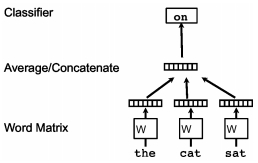
\includegraphics[width=1\textwidth]{img/par2vec_arq}
\caption{Paragraph vector PV-DM architecture.}
\label{fig:p2v_arq}
\end{minipage}
\end{figure}

Once the model is trained, it can be queried so as to get the vector representations for each already seen sentence. It can also be used to \emph{infer} vector mappings of \emph{unseen} sentences. This second step will be crucial to get representations for utterances in our test dataset.

A great advantage of these approach is that it is completely unsupervised, and thus, we can use any amount of unlabelled data we want.

\subsubsection*{Word2vec pretrained vectors}
The implementation we use for getting paragraph vectors allows us to use already existing word embeddings. The way in which this feature works is as follows: (a) No new words are added to the vocabulary; (b) Intersecting words adopt pretrained values ; (c) Non intersecting words are left alone.
For our experiments, we try both alternatives, training word and paragraph embeddings from scratch using several dialog corpora as input, and also using freely available embeddings\footnote{\url{https://code.google.com/p/word2vec/}}.

\subsection{Dialog datasets}
\lau{Describe the switchboard corpus. It's 42 tags.}
\lau{Describe the BNC corpus.}

\subsubsection*{The Switchboard corpus}

\subsubsection*{The British National corpus}

\subsection{Classifiers}
\lau{Mention which classifiers we use, and with which params}